\section{Übersicht} \label{sec:Übersicht}
\begin{center}
	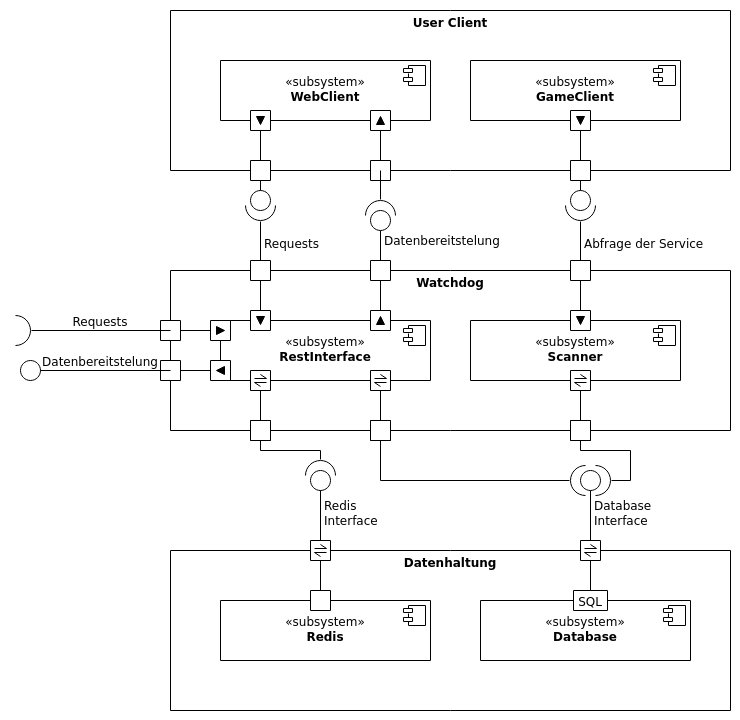
\includegraphics[width=\linewidth, keepaspectratio]{entwurf/uebersicht_component}
	\captionof{figure}{Übersicht über die Anwendung (Komponentendiagramm)}
	\label{fig:system-overview}
\end{center}

Die Gesamtheit des Systems (inklusive der User Clients), wie in Abbildung \ref{fig:system-overview} zu sehen, lässt sich in drei Ebenen einteilen.

\paragraph{User Client}
Die erste Ebene \textit{User Client} beinhaltet die auf einem User Client laufende für den Versuch relevanten Komponenten.

Bei der Komponente Webclient handelt es sich um einen geläufigen Webbrowser (häufig wird Firefox genutzt), welcher Informationen vom \textit{CTF Core System} abruft und Daten an dieses übermittelt.
Zu den Informationen gehören beispielsweise die Spielinformationen, der Spielstand aber auch teilnehmende Gruppen und Einstellungen. Der Webclient übermittelt Daten, wie gefundene Flags, Lösungen von Aufgaben und Änderungen an Einstellungen.

Die Komponente \textit{GameClient} beinhaltet alle auf dem System für den Versuch installierten Anwendungen. Dazu zählen nicht nur die Dienste mit den Schwachstellen. Auch die clientseitige Spielverwaltungs-Software wird unter dieser Komponente zusammengefasst. Die Spielverwaltungs-Software sorgt für die richtige Konfiguration des User Clients und versteckt die Flags.

\paragraph{CTF Core System}
Die Ebene des \textit{CTF Core System} besteht aus zwei Komponenten. 

Zum einen aus der Komponente \textit{Big Brother}. In der Komponente ist die Überwachung des \textit{GameClients} mit seinen Schwachstellen implementiert. Die Ergebnisse dieser Überwachung werden in der \textit{Database} festgehalten.

Zum anderen aus der Komponente \textit{Game Information System}. Diese stellt eine Schnittstelle zwischen der Datenbank und den Nutzern dar. Mithilfe der Schnittstelle können Informationen unter Berücksichtigung von Berechtigungen auf einem einheitlichen Weg aus der Datenbank ausgelesen, verändert und hinzugefügt werden. 

\paragraph{Datenhaltung}
Die Ebene \textit{Datenhaltung} beinhaltet die Komponenten \textit{Redis} und \textit{Database}. 

Die Komponente \textit{Redis} ist nach der gleichnamigen Software Redis benannt. Bei Redis handelt es sich auch um eine Datenbank und könnte daher mit in der Komponente \textit{Database} aufgenommen werden, die Trennung erfolgt, aber auf Grundlage der Verwendung innerhalb der Software Architektur. Die Redis-Datenbank wird als Cache verwendet und persistiert die Daten nicht.

Anderes als bei Redis werden in der Komponente \textit{Database} die Daten auf eine Festplatte festgeschrieben um, diese persistent nutzen zu können.